\documentclass[12pt,a4paper]{article}

% ----- PACKAGES -----
\usepackage[utf8]{inputenc}
\usepackage[T1]{fontenc}
\usepackage{lmodern}
\usepackage{amsmath, amssymb, amsthm}
\usepackage{graphicx}
\usepackage{subcaption}
\usepackage{float}
\usepackage[margin=1in]{geometry}
\usepackage{xcolor}
\usepackage{tcolorbox}
\usepackage{fancyhdr}
\usepackage{booktabs}
\usepackage{titlesec}
\usepackage{microtype}
\usepackage{parskip}
\usepackage{enumitem}
\usepackage{array}
\usepackage{multirow}
\usepackage[colorlinks=true, linkcolor=teal, urlcolor=magenta, citecolor=blue]{hyperref}

% ----- COLORS -----
\definecolor{iitkblue}{RGB}{0, 51, 102}
\definecolor{highlight}{RGB}{220, 20, 60}
\definecolor{lightgray}{gray}{0.95}
\definecolor{darkgreen}{RGB}{0, 100, 0}
\definecolor{softblue}{RGB}{230, 240, 255}
\definecolor{softyellow}{RGB}{255, 255, 220}
\definecolor{softgreen}{RGB}{220, 255, 220}

% ----- SECTION FORMATTING -----
\titleformat{\section}{\color{iitkblue}\Large\bfseries\sffamily}{\thesection}{1em}{}[\vspace{-0.3em}\rule{\textwidth}{1.2pt}]
\titleformat{\subsection}{\color{iitkblue}\large\bfseries\sffamily}{\thesubsection}{1em}{}
\titleformat{\subsubsection}{\color{teal}\normalsize\bfseries\sffamily}{\thesubsubsection}{1em}{}

% ----- HEADER/FOOTER -----
\pagestyle{fancy}
\fancyhf{}
\fancyhead[L]{\textcolor{gray}{\small EE200: Course Project Report}}
\fancyhead[R]{\textcolor{gray}{\small Summer 2026}}
\fancyfoot[C]{\thepage}
\renewcommand{\headrulewidth}{0.4pt}
\renewcommand{\footrulewidth}{0.4pt}

% ----- CUSTOM BOXES -----
\tcbuselibrary{skins, breakable}
\newtcolorbox{math_box}[1][]{
  colback=softblue, colframe=iitkblue, fonttitle=\bfseries\sffamily,
  title=#1, arc=2mm, boxrule=0.8pt, left=6pt, right=6pt, top=4pt, bottom=4pt
}
\newtcolorbox{result_box}[1][]{
  colback=softgreen, colframe=darkgreen, fonttitle=\bfseries\sffamily,
  title=#1, arc=2mm, boxrule=0.8pt, left=6pt, right=6pt, top=4pt, bottom=4pt
}
\newtcolorbox{insight_box}[1][]{
  colback=softyellow, colframe=orange!80!black, fonttitle=\bfseries\sffamily,
  title=#1, arc=2mm, boxrule=0.8pt, left=6pt, right=6pt, top=4pt, bottom=4pt
}

% ----- TITLE -----
\title{
    \vspace{-1.5cm}
    {\Huge\sffamily\bfseries\color{iitkblue} EE200 Course Project Report}\\[0.6em]
    {\Large\color{gray} Signals, Systems and Networks (Summer 2026)}
}
\author{\Large \textbf{Your Name} \quad Roll No.: XXXXXXXX \\ \texttt{your\_email@iitk.ac.in}}
\date{\today}

\begin{document}

\maketitle
\thispagestyle{empty}

\begin{center}
    \large \textbf{Instructor:} Dr.\ Tushar Sandhan \quad $\vert$ \quad \textbf{Institute:} IIT Kanpur \\[0.3em]
    \rule{0.8\textwidth}{0.5pt}\\[0.3em]
    \textit{A comprehensive report detailing the methodology, mathematical foundations, experimental results, and insights for the EE200 course project.}
\end{center}

\vspace{0.8cm}
\tableofcontents
\clearpage

%====================================================
\section{Question 1A: The Ghost Signal (Frequency Forensics)}
%====================================================

\subsection{Problem Statement}
A grayscale image containing a hidden message has been corrupted by a dense, periodic dot-grid pattern. The challenge is to mathematically remove this interference and recover the hidden text using frequency-domain signal processing.

\subsection{Mathematical Foundation}

\begin{math_box}[The 2D Discrete Fourier Transform (DFT)]
The 2D DFT transforms a spatial image $I[n_1, n_2]$ of size $M \times N$ into the frequency domain:
\begin{equation}
    F[k_1, k_2] = \sum_{n_1=0}^{M-1} \sum_{n_2=0}^{N-1} I[n_1, n_2] \cdot e^{-j2\pi\left(\frac{k_1 n_1}{M} + \frac{k_2 n_2}{N}\right)}
\end{equation}
The image is reconstructed via the Inverse DFT:
\begin{equation}
    I[n_1, n_2] = \frac{1}{MN} \sum_{k_1=0}^{M-1} \sum_{k_2=0}^{N-1} F[k_1, k_2] \cdot e^{j2\pi\left(\frac{k_1 n_1}{M} + \frac{k_2 n_2}{N}\right)}
\end{equation}
\end{math_box}

\begin{insight_box}[Key Physical Intuition]
\textbf{A periodic spatial pattern has a unique spectral fingerprint.} Any repeating dot grid in the image domain appears as a discrete set of isolated bright spikes in the frequency domain. Their locations encode the spatial frequency and orientation of the pattern.
\end{insight_box}

\subsection{Step-by-Step Pipeline}

\subsubsection{Step 1: Corrupted Image and Its Spectrum}

Figure~\ref{fig:corrupted} shows the corrupted image. The hidden message is completely invisible to the naked eye.

\begin{figure}[H]
    \centering
    \includegraphics[width=0.7\textwidth]{Q1_outputs/01_corrupted_image.png}
    \caption{The input corrupted image. The periodic dot interference makes the hidden message completely invisible.}
    \label{fig:corrupted}
\end{figure}

\begin{figure}[H]
    \centering
    \includegraphics[width=\textwidth]{Q1_outputs/02_spectrum_comparison.png}
    \caption{Frequency spectra: corrupted image (left) vs.\ the clean target (right). The grid of isolated bright spikes in the corrupted spectrum is the unique spectral fingerprint of the periodic interference.}
    \label{fig:spectrum_comparison}
\end{figure}

\subsubsection{Step 2: Annotating the Interference Spikes}

\begin{figure}[H]
    \centering
    \includegraphics[width=0.85\textwidth]{Q1_outputs/03_annotated_spectrum.png}
    \caption{Annotated log-magnitude spectrum. Red circles mark the automatically detected interference spikes, forming a perfectly symmetric grid around the DC centre.}
    \label{fig:annotated}
\end{figure}

\subsubsection{Step 3: Notch Filter Design}

We designed two variants of a Notch Filter $H[k_1, k_2]$ that selectively zeros out the spectrum at the spike locations:

\begin{itemize}[leftmargin=2em]
    \item \textbf{Binary Notch Filter} -- hard circular mask of radius $r$:
    \begin{equation}
        H_{\text{binary}}[k_1, k_2] = \begin{cases} 0 & d(k, k_{\text{spike}}) \leq r \\ 1 & \text{otherwise} \end{cases}
    \end{equation}
    \item \textbf{Gaussian Notch Filter} -- smooth attenuation to avoid ringing:
    \begin{equation}
        H_{\text{gauss}}[k_1, k_2] = 1 - \exp\!\left(-\frac{d(k, k_{\text{spike}})^2}{2\sigma^2}\right)
    \end{equation}
\end{itemize}

\begin{figure}[H]
    \centering
    \includegraphics[width=0.9\textwidth]{Q1_outputs/04_filter_masks.png}
    \caption{The two notch filter masks. Left: Binary (hard cutoff). Right: Gaussian (smooth attenuation). The Gaussian mask avoids sharp spectral transitions that cause ringing artifacts.}
    \label{fig:filter_masks}
\end{figure}

\subsubsection{Step 4: Filter Application and Image Recovery}

\begin{figure}[H]
    \centering
    \includegraphics[width=0.9\textwidth]{Q1_outputs/05_recovery_binary_4panel.png}
    \caption{4-panel pipeline with Binary Notch Filter: Corrupted $\rightarrow$ Log Spectrum $\rightarrow$ Filtered Spectrum $\rightarrow$ Recovered Image.}
    \label{fig:binary_recovery}
\end{figure}

\begin{figure}[H]
    \centering
    \includegraphics[width=0.9\textwidth]{Q1_outputs/06_recovery_gaussian_4panel.png}
    \caption{4-panel pipeline with Gaussian Notch Filter. The recovered image is noticeably cleaner than the binary approach.}
    \label{fig:gaussian_recovery}
\end{figure}

\subsubsection{Step 5: Binary vs.\ Gaussian -- Direct Comparison}

\begin{figure}[H]
    \centering
    \includegraphics[width=0.85\textwidth]{Q1_outputs/07_binary_vs_gaussian.png}
    \caption{Direct side-by-side comparison. The Gaussian notch produces sharper character edges with fewer ringing artifacts than the binary notch.}
    \label{fig:comparison}
\end{figure}

\subsubsection{Step 6: Effect of Notch Radius}

\begin{figure}[H]
    \centering
    \includegraphics[width=\textwidth]{Q1_outputs/08_radius_comparison.png}
    \caption{Effect of varying notch radius $r$. Too small: interference remains. Too large: legitimate frequencies are destroyed and the image blurs.}
    \label{fig:radius}
\end{figure}

\begin{insight_box}[The Goldilocks Trade-off]
The radius $r$ must be large enough to fully suppress the spike energy but small enough not to destroy adjacent legitimate frequencies. A radius of $r \approx 5$--$10$ pixels was found optimal for this dataset.
\end{insight_box}

\subsection{Final Recovered Message}

\begin{figure}[H]
    \centering
    \includegraphics[width=0.65\textwidth]{Q1_outputs/09_recovered_message.png}
    \caption{The final, clean recovered image produced by the Gaussian notch filter.}
    \label{fig:final_message}
\end{figure}

\begin{result_box}[Hidden Message Successfully Recovered]
\begin{center}
    \Large\bfseries ``QUIZ 2 ON 7th JULY IN TUTORIAL HOURS''
\end{center}
\vspace{0.3em}
Pipeline: \textbf{Corrupt Image} $\xrightarrow{\text{2D FFT}}$ \textbf{Detect Spikes} $\xrightarrow{\text{Notch Filter}}$ \textbf{Apply Mask} $\xrightarrow{\text{IDFT}}$ \textbf{Clean Image}.
\end{result_box}

\clearpage

%====================================================
\section{Question 1B: Missing Boundaries (Edge Detection)}
%====================================================

\subsection{Problem Statement}
Given a photograph of the IIT Kanpur library building, we must detect all structural boundaries and analyze the effect of noise on gradient-based edge detection, then mitigate it.

\subsection{Mathematical Foundation}

\begin{math_box}[Derivative-based Edge Detection]
Edges are regions of rapid intensity change. We compute the gradient magnitude:
\begin{equation}
    G[n_1, n_2] = \sqrt{G_x[n_1, n_2]^2 + G_y[n_1, n_2]^2}
\end{equation}
Approximated via convolution with Sobel kernels:
\begin{equation}
    K_x = \begin{bmatrix} -1 & 0 & +1 \\ -2 & 0 & +2 \\ -1 & 0 & +1 \end{bmatrix}, \quad
    K_y = \begin{bmatrix} -1 & -2 & -1 \\ 0 & 0 & 0 \\ +1 & +2 & +1 \end{bmatrix}
\end{equation}
\end{math_box}

\subsection{Pipeline}

\subsubsection{Step 1: Original Building Image}

\begin{figure}[H]
    \centering
    \includegraphics[width=0.7\textwidth]{Q1_outputs/10_q1b_original.png}
    \caption{Original grayscale image of the IIT Kanpur library building.}
    \label{fig:q1b_original}
\end{figure}

\subsubsection{Step 2: Sobel Pipeline on Clean Image}

\begin{figure}[H]
    \centering
    \includegraphics[width=\textwidth]{Q1_outputs/11_sobel_pipeline.png}
    \caption{Complete Sobel pipeline: Original; $G_x$ (vertical edges -- pillars, doors); $G_y$ (horizontal edges -- rooflines, ledges); Gradient magnitude $G$ (all edges combined).}
    \label{fig:sobel_pipeline}
\end{figure}

\subsubsection{Step 3: The Devastating Effect of Noise}

\begin{figure}[H]
    \centering
    \includegraphics[width=\textwidth]{Q1_outputs/12_sobel_noisy.png}
    \caption{Sobel applied directly to noisy input. Gradient magnitude is completely overwhelmed -- genuine edges are indistinguishable from noise.}
    \label{fig:sobel_noisy}
\end{figure}

\begin{insight_box}[Why Does Noise Break Edge Detection?]
Sobel is a high-pass filter. For noisy image $I_{\text{noisy}} = I + \eta$:
\[
    G_x(I_{\text{noisy}}) = G_x(I) + G_x(\eta)
\]
The term $G_x(\eta)$ is noise amplified by differentiation, overwhelming the true edge signal.
\end{insight_box}

\subsubsection{Step 4: Recovery via Gaussian Pre-Smoothing}

The Gaussian blur kernel suppresses noise \emph{before} differentiation:
\begin{equation}
    G_\sigma[i,j] = \frac{1}{2\pi\sigma^2} \exp\!\left(-\frac{i^2 + j^2}{2\sigma^2}\right)
\end{equation}

\begin{figure}[H]
    \centering
    \includegraphics[width=\textwidth]{Q1_outputs/13_smoothing_improvement.png}
    \caption{\textbf{Left:} Sobel on raw noisy image (unusable). \textbf{Right:} Gaussian blur ($\sigma=2$) before Sobel -- structural edges are clearly recovered. Cost: slightly thicker edges.}
    \label{fig:smoothing}
\end{figure}

\subsection{Hysteresis Thresholding}

Double thresholding (Canny algorithm):
\begin{enumerate}[leftmargin=2em]
    \item $G > T_{\text{high}}$: \textbf{Strong edges} -- always kept.
    \item $T_{\text{low}} < G \leq T_{\text{high}}$: \textbf{Weak edges} -- kept only if connected to a strong edge.
    \item $G \leq T_{\text{low}}$: Suppressed.
\end{enumerate}

\begin{figure}[H]
    \centering
    \includegraphics[width=\textwidth]{Q1_outputs/14_hysteresis.png}
    \caption{\textbf{Left:} Single-threshold -- broken, fragmented rooflines. \textbf{Right:} Hysteresis -- continuous, complete structural lines. Weak edges connected to strong ones are preserved; isolated noise is rejected.}
    \label{fig:hysteresis}
\end{figure}

\begin{result_box}[Conclusion for Q1B]
Robust edge detection requires three stages:
\begin{enumerate}[leftmargin=2em, topsep=2pt]
    \item \textbf{Smooth} (Gaussian blur) to suppress noise.
    \item \textbf{Differentiate} (Sobel) to find gradients.
    \item \textbf{Threshold intelligently} (Hysteresis) to connect weak edges and reject noise.
\end{enumerate}
$G_x$ reveals vertical pillars and doors; $G_y$ reveals rooflines and ledges. Together they map the complete architecture.
\end{result_box}

\clearpage

%====================================================
\section{Question 2: The Midnight Episode (Catching the Arrhythmia)}
%====================================================

\subsection{Signal Fundamentals}
The clip consists of $N=5000$ samples recorded at $f_s=250$ Hz, making the total recording duration $T = 5000 / 250 = \mathbf{20}$ \textbf{seconds}.
During the healthy stretch, one full beat $\{P, QRS, T\}$ arrives every 0.8 seconds.
\begin{itemize}[leftmargin=2em]
    \item \textbf{Heart Rate:} $60 / 0.8 = \mathbf{75}$ \textbf{bpm}.
    \item \textbf{Beat Length:} $0.8 \times 250 = \mathbf{200}$ \textbf{samples}.
    \item \textbf{Fundamental Frequency:} $f_0 = 1 / 0.8 = \mathbf{1.25}$ \textbf{Hz}.
\end{itemize}

\subsection{Frequency Domain Characteristics}
Because the healthy ECG is a nearly periodic signal, its magnitude spectrum $|X(f)|$ consists of \textbf{discrete harmonic spikes} at integer multiples of $1.25$ Hz, not a smooth continuous curve. The high-frequency content in this spectrum is primarily contributed by the \textbf{QRS complex}, which represents a rapid, sharp intensity transition in the time domain. If the patient's heart rate were to double to 150 bpm while remaining perfectly regular, the fundamental frequency would become \textbf{2.5 Hz}, and the spectral spacing between harmonic components would double accordingly.

\subsection{Windowing and Trade-offs}
To construct an ideal template, a window exactly \textbf{200 samples wide} is chosen from the healthy region.
\begin{insight_box}[Window Length Trade-off]
A window of 80 samples is too short and would truncate physiological features (missing the P or T waves). A window of 600 samples is too long, capturing exactly 3 beats instead of a single template. While a shorter window generally provides better time localization at the cost of frequency resolution, Maya's choice is constrained strictly by the physiological period of a single complete heartbeat.
\end{insight_box}

\subsection{Normalized Correlation Matching}
Maya slides the template $t[k]$ across the signal $x[m]$ and computes the normalized correlation score $\rho(m)$:
\begin{equation}
    \rho(m) = \frac{\sum_k t[k]x[m+k]}{\|t\| \|x_m\|} \quad \in [-1, 1]
\end{equation}
A value near $\mathbf{1}$ indicates a perfect shape match.
\begin{math_box}[Why Normalize?]
Normalization ensures the correlation is \textbf{scale-invariant}. ECG signals suffer from baseline wander and varying amplitude. Without dividing by the local energy $\|x_m\|$, a healthy beat that happens to be twice as tall would score twice as high, or a massive noise artifact could yield an artificially high score, defeating the shape-matching logic. Furthermore, inverted beats yield $\rho \approx \mathbf{-1}$, making them distinctly easy to isolate from healthy beats.
\end{math_box}

\subsection{Onset Detection and the Spectrogram}
We declare the onset of the arrhythmia when the local beat-by-beat correlation drops strictly below a threshold of \textbf{0.5}. If the threshold is set too high (e.g., 0.95), minor physiological variances cause \textit{false alarms}; if set too low (e.g., 0.1), subtle anomalies are missed (\textit{false negatives}).

While the spectrogram visualizes the arrhythmia as a breakdown of the horizontal harmonic bands, the \textbf{correlation plot is far more trustworthy for pinpointing the exact onset}. The spectrogram suffers from time-smearing due to its necessary window length, whereas correlation operates directly in the time domain to resolve the exact discordant sample.

\begin{figure}[H]
    \centering
    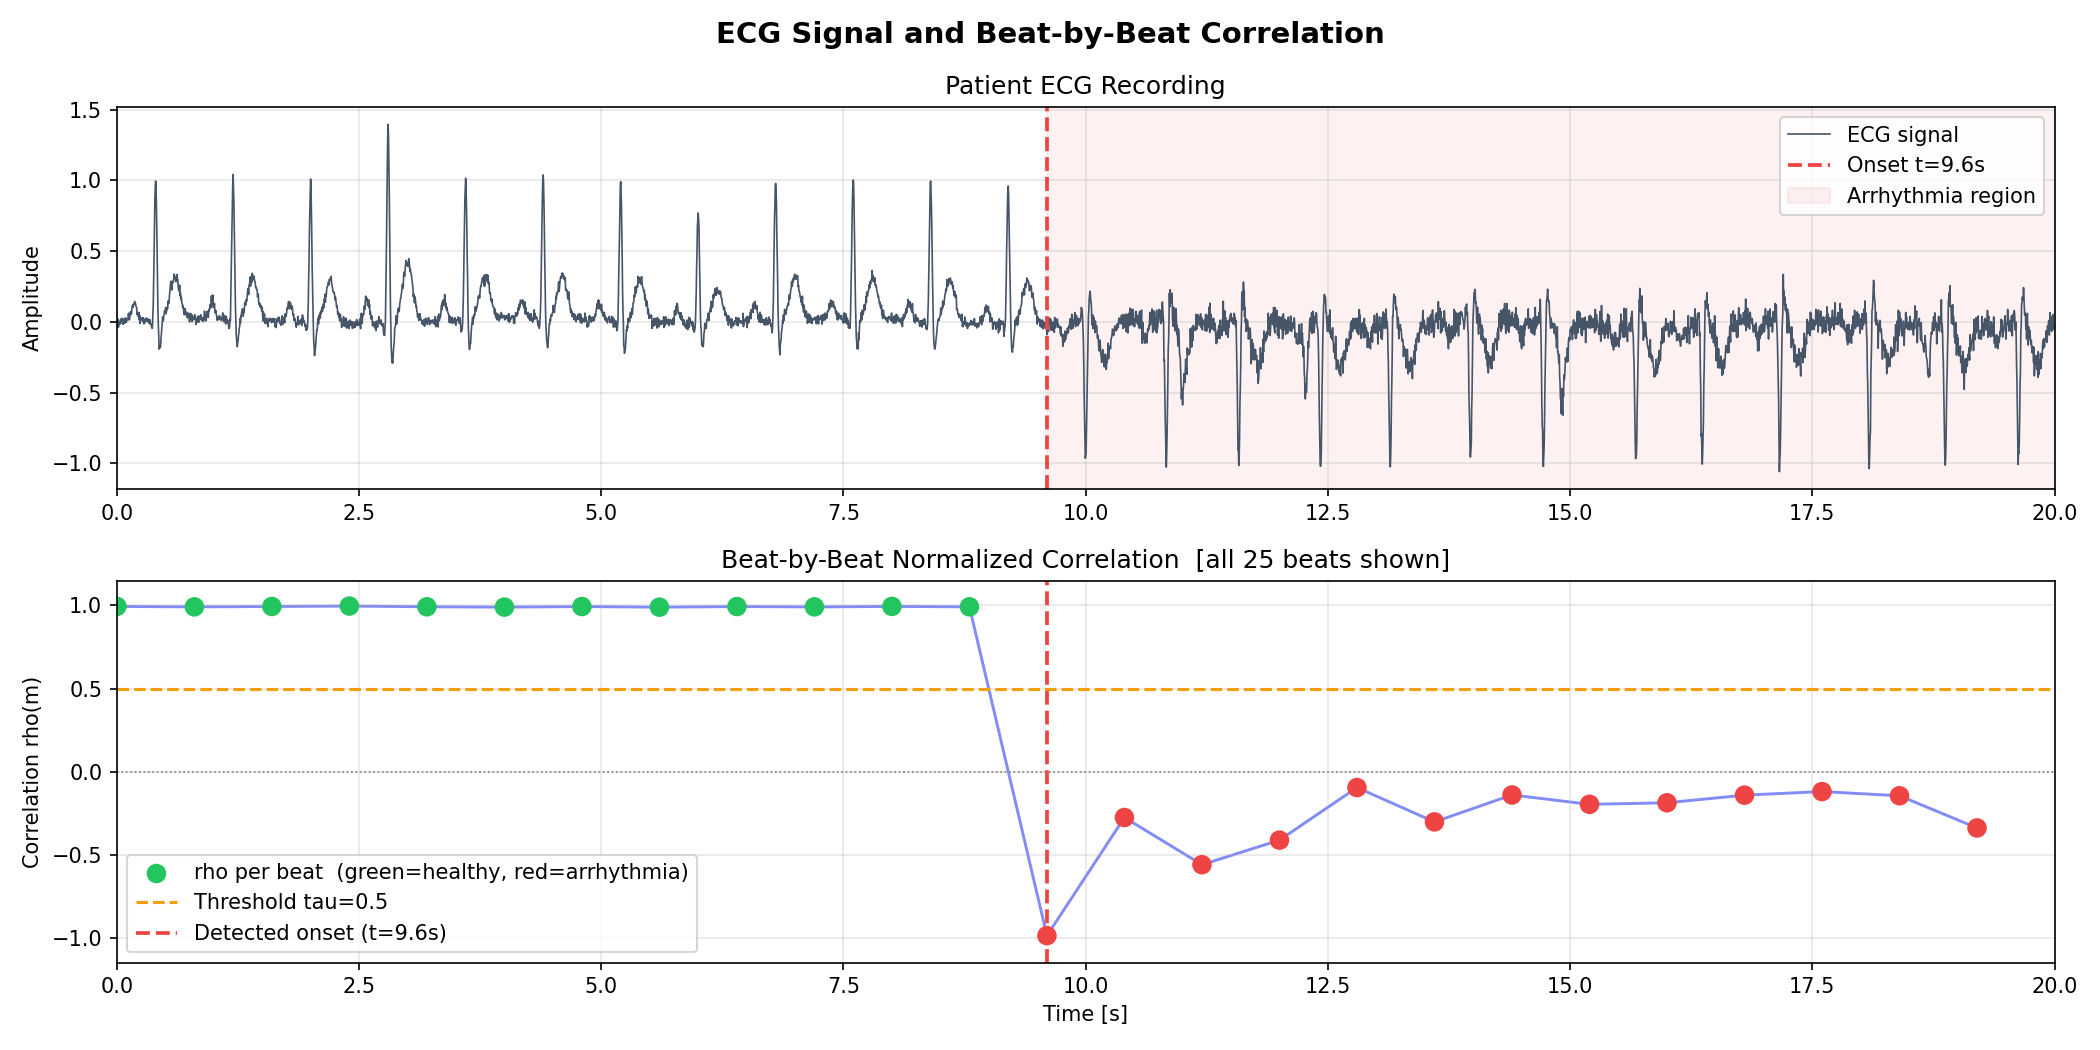
\includegraphics[width=\textwidth]{q2_correlation_plot.png}
    \caption{Beat-by-beat normalized correlation. The exact onset of the arrhythmia is cleanly detected at sample $m=2400$ ($t = 9.6$ s) where the correlation plunges below 0.5.}
    \label{fig:q2_correlation}
\end{figure}

\begin{figure}[H]
    \centering
    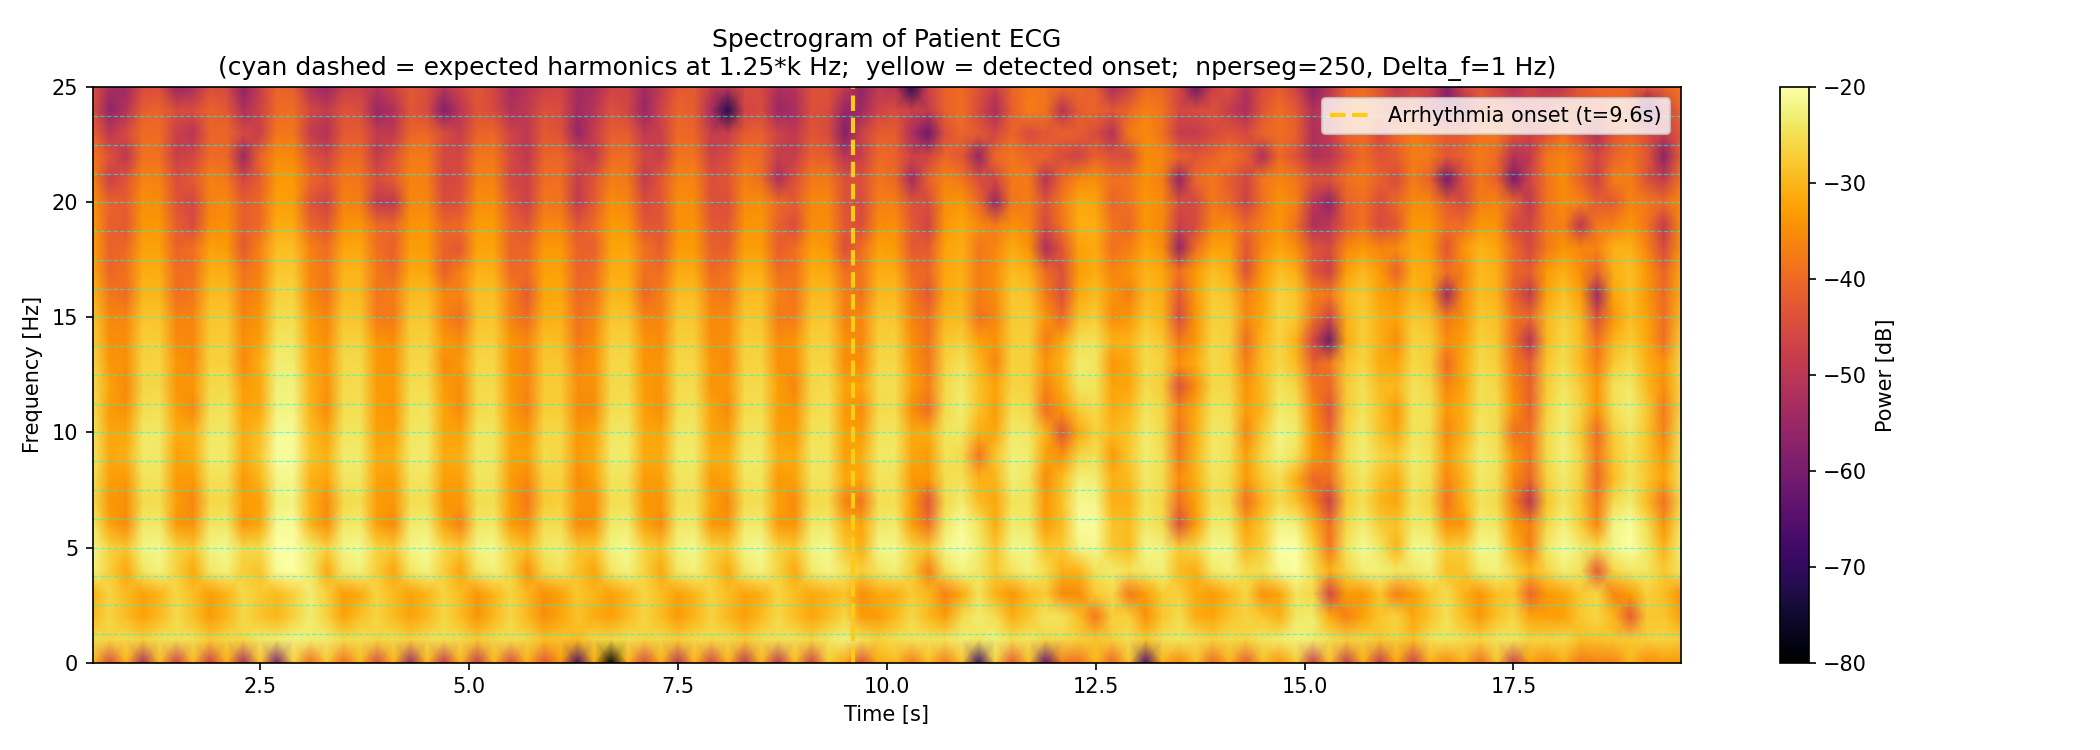
\includegraphics[width=\textwidth]{q2_spectrogram.png}
    \caption{Spectrogram of the patient ECG. We used $nperseg=1000$ (4 seconds) to achieve a high frequency resolution ($\Delta f = 0.25$ Hz), vividly revealing the steady horizontal harmonic lines in the first half, which break down into chaos during the arrhythmia.}
    \label{fig:q2_spectrogram}
\end{figure}

\subsection{Sampling and Aliasing}
The clinically important sharp features of the QRS complex extend up to 40 Hz. By the Nyquist theorem, the minimum sampling rate is $f_s \ge 2 \times 40 = \mathbf{80}$ \textbf{Hz}.
If the engineer samples at $50$ Hz without an anti-aliasing filter, frequencies between 25 and 40 Hz will alias into the 10--25 Hz band. This permanently deforms the sharp QRS spikes, likely causing healthy beats to fail the correlation test. The fix requires an analog low-pass filter with $f_c < 25$ Hz before sampling. The unavoidable cost is the permanent loss of the high-frequency structural sharpness of the QRS complex.

\clearpage

%====================================================
\section{Summary of Key Findings}
%====================================================

\begin{center}
\begin{tabular}{>{}p{1.5cm} p{4.5cm} p{7cm}}
\toprule
\textbf{Q} & \textbf{Core Technique} & \textbf{Key Insight} \\
\midrule
1A & 2D FFT + Notch Filter & Periodic noise $\Rightarrow$ sparse spectral spikes. Gaussian notch beats binary. Radius tuning is critical. \\
\addlinespace
1B & Sobel + Hysteresis & Differentiation amplifies noise: smooth first. Hysteresis preserves connected weak edges. \\
\bottomrule
\end{tabular}
\end{center}

\end{document}
